\section{Evaluation and results}\label{sec:evaluation}
We evaluate the policy every \(10\) collector batches in a deterministic modes, by taking the mode of the the policy distribution. 
%Evaluation may have a different rollout length, but in any case (\(\geq \max(l,m)\)). 
The evaluation starts at random polynomials with up to \(3\) non zero elements (similarly to training). 
Every step of every evaluation is logged, giving, per evaluation, the full trajectory of rewards and of the constructed codes. 
The following \emph{metrics} are observed:
\paragraph{Best-performing code} We are interested, of course, in maximising the reward under a given decoder. For known, published, code parameters, we can calculate this number and measure against it.
\paragraph{80\% of the evaluation} This is of interest because it helps understand whether the agent is actually improving, in which case the 80\% band will tighten in width, and tighten the gap with the maximum. 
A persistent gap between the band and the maximum means the best
codes visited are fewer than $10\%$ of the time, implying that discovered good codes are not integrated into the policy. 
A persistently wide 80\% band is a proxy metric to 
\textit{how many steps did it take the agent to reach the best code ?} 
as an all knowing agent would plot a reward-greedy course towards the best code. The best code (the reference published code) is at most \(max{l,m}\) actions far, 
but potentially goes through some bad-paying codes. This is why we look at the fraction of steps the agent spent in \(5\) regions:
\begin{enumerate}[label = \roman*]
        \label{list:regions}
\item \textbf{Invalid codes}
\item Codes that yielded \textbf{0-50\%} of the reference reward
\item Codes that yielded \textbf{50-95\%} of the reference reward
\item Codes that yielded \textbf{95-100\%} of the reference reward
\item Codes that yielded a reward equal to or greater than the reference.
\end{enumerate}

\paragraph{Average reward} The average reward can indicate whether or not the agent has learned that codes with insufficient number of logical qubits obtain a negative reward.
\paragraph{Within-episode gain} This is the difference between the the reward for the code the envornoment \bfit{reset} into, and the \bfit{last} code the agent arrived in. Where learning was succesful, we expect this value to increase over time. 
This metric helps to filter out any episodes where the agent received a ``lucky'' reset value, and 

\noindent Figure~\ref{fig:reward-panel} summarises several metrics, carried over \bfit{one} training run. We use the codes reported in~\cite{bravyi2024high} as 
baselines. Where a baseline code exists, we plot the reward this code would achieve as a reference (horizontal, gray, dashed). The shaded region below zero reward marks where the reward was negative due to a code with less than the minimum number of logical qubits required, 
and the exact number of logical qubits can be recovered from the negative reward (annotated next to the reward ticks). A dashed vertical line indicates when the encoder weights were unfrozen. Within each evaluation we plot the \bfit{best} (maximum) reward obtained (blue), the \bfit{average} (orange), 
and the 10th to 90th percentile of the rewards obtained in that evaluation in shaded orange\footnote{Which will always be around the average and below the maximum.}, which indicates where 80\% of that evaluation was spent.

\paragraph{Anatomy of a single run}
\begin{figure*}[htbp]
    \centering
    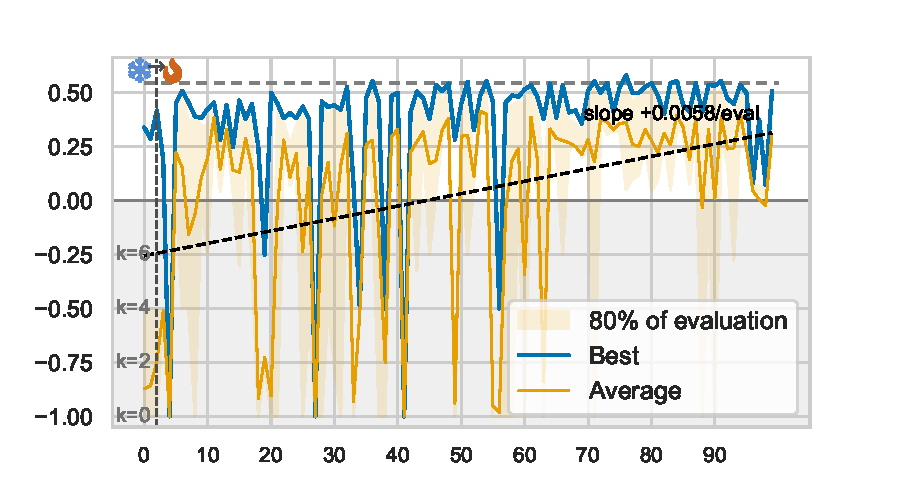
\includegraphics[width=\linewidth]{art/evaluation/paper_2026-08-03_19-34-15_1777554.pdf}
    \caption{Evaluation of a single PPO training session. Horizontal dashed line marks the reward for a published reference code (which is expected to be the maximum possible reward). Vertical dashed line marks when the encoder weights were unfrozen \faSnowflake{} $\rightarrow$ \faFire{}. As learning progresses, the 80\% band (transparent orange) is contracts towards the best codes in the evaluation and lifts off from the penalty region (shaded lower part).}
    \label{fig:reward-panel}
\end{figure*}
Early in training the 80\% band is high-spread and sits largely inside the penalty region (shaded gray) and the agent spends most of its steps climbing from the random reset 
code towards codes with more logical qubits. 
As training progresses, a successful run shows the band shifting away from the penalty region. 
As training matures, we see the best-in-evaluation line (blue) crossing the reference more consistently. 
We also see that the 80\% band contracts later in training. A deep dip accompanied by a high-spread band is a
slow recovery, suggesting the evaluation started from an unfavourable and the agent was slow to recover. 
A dip whose band is tightly centered around $-1$ suggests a trapped evaluation, i.e., the deterministic policy cannot climb out of the penalty region.
Recall that evaluations are deterministic. A trapped evaluation reflects a property
of the greedy policy from that particular initial code. The training time
policy, which samples with an entropy bonus, wouldn't necessarily fail from the same state, but such an event shows a weakness of the deterministic policy. 
These observations can be seen in Figure~\ref{fig:reward-panel}.


\paragraph{Analysis of multiple runs}
Figure~\ref{fig:multiple96} (left) show a stacked plot of where the agent spends evaluation time divided by the 
regions~\ref{list:regions}, for \(28\) runs for the \(9,6\) parameters (multiple seeds, multiple encoders). 
As training progresses, the agent spends less time on codes that have less the minimum required number of logical qubits.
\begin{figure*}
        \centering
        \begin{subfigure}{0.48\linewidth}
        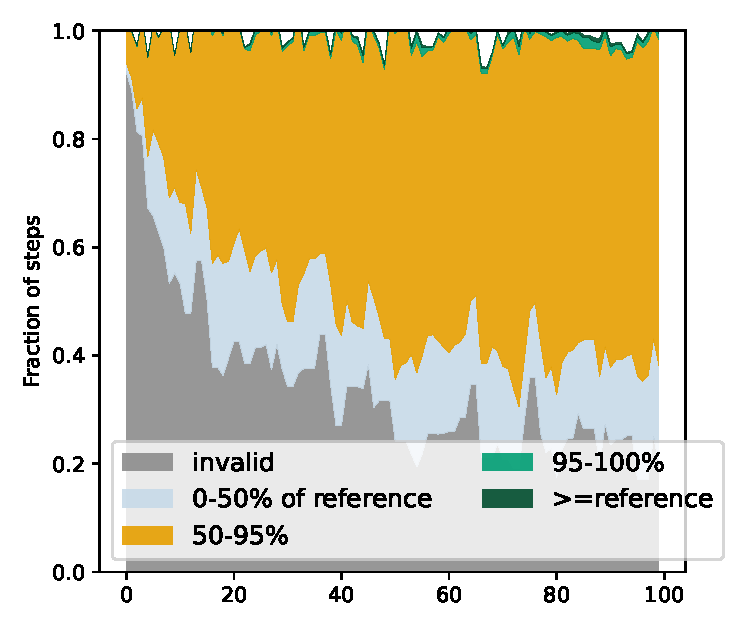
\includegraphics[width=\linewidth]{art/evaluation/multiple_runs_l_9_m_6_month_August_eval_rollout_length_30_where_spent.pdf}
        \end{subfigure}
        \hfill
        \begin{subfigure}{0.48\textwidth}
        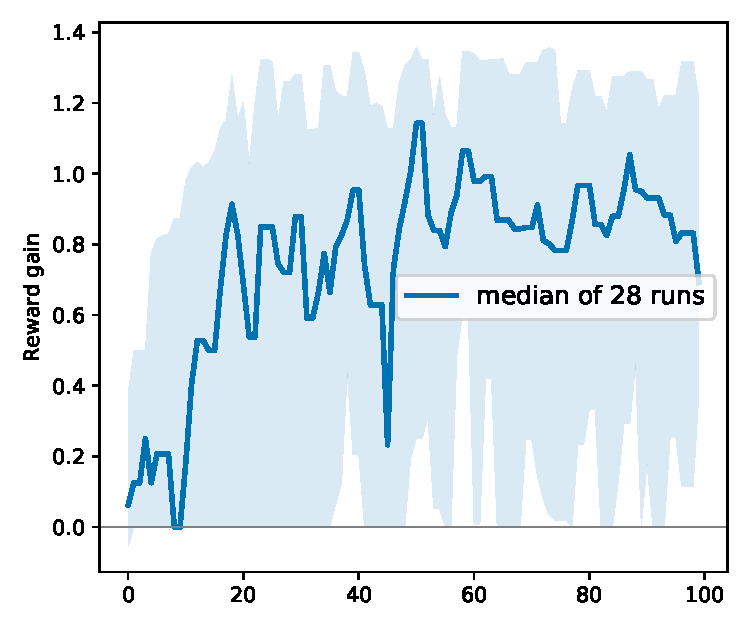
\includegraphics[width=\linewidth]{art/evaluation/multiple_runs_l_9_m_6_month_August_eval_rollout_length_30_episode_gain.pdf}

        \end{subfigure}
                \caption{Left: stacked plot corresponding to the regions defined in \ref{list:regions}. The reference code is considered the best possible. As training progresses, the agent spends more of the evaluation time in better performing regions. 
                Right: rolling median (pooled over one adjacent evaluation on either side) within-episode gain, calculated as the difference between the reward for the first and last code of the episode.}
        \label{fig:multiple96}
\end{figure*}
\noindent Figure~\ref{fig:multiple96} (right) shows the median episode gain for the same \(28\) runs of the \(9,6\) 
code, with a 50\% band. As learning progresses, the median gain within episode increases up to evaluation \(50\), where it begins to stabilise. The reward for the reference code can be found in Table~\ref{tab:configuration}, \(0.546\) for the \(9,6\) code.
\subsection{Evaluation of the network architecture\label{sec:validation}}
Recall that our network architecture in Section~\ref{sec:policy} proposed three branches, with the main ones being the MLP (which number of parameters depend on the size of the code) 
and the encoder (which is transferable across code sizes). Furthermore, in Section~\ref{sec:critic} we proposed using a pretrained encoder, which, depending on what the agent struggles on, could warm-start the learning.
As Table~\ref{tab:kCurveAlignment} suggests, it is hard to pick an encoder that excels both tasks.
The selection therefore had to be done once we learned whether the agent struggles (at early training) with getting to codes with sufficient number of logical qubits, 
or whether it struggles to find good codes which meet the threshold. 
We can, however, review some training strategies, assuming we find an encoder that compensates for early start stagnation (yet to be demonstrated).
Looking at Figure~\ref{fig:reward-panel}, as well as the breakdown of Figure~\ref{fig:multiple96} (left), 
suggests that it is learning to produce codes with a sufficient number of qubits that the agent struggles with at first.
We therefore chose encoders that excelled at predicting the number of logical qubits of a code.
To test whether a pretrained encoder can improve sampling efficiency, we used identical PPO hyperparameters and seeds, 
and plot in Figure~\ref{fig:unfreezeSweep} the fraction of time spent at invalid codes, as a function of the unfreeze index (the episode from which the encoder weights are unfrozen).
\begin{figure}
        \centering
        \includegraphics[width = 0.8\textwidth]{art/encoder/unfreezeExperiment.pdf}
        \caption{Fraction of the evaluation spent at codes that had less than the minimum required logical qubits.}
        \label{fig:unfreezeSweep}
\end{figure}
The results in Figure~\ref{fig:unfreezeSweep} show that any delay in unfreezing the encoder weights, produces higher stagnation of the agent, meaning, more time  spent in codes that score a negative reward. 
In simple terms, sampling efficiency degrades as unfreeze is delayed.
%Adding this to the tension in Table~\ref{tab:kCurveAlignment}
% \paragraph{Warm-started} the architecture of Figure~\ref{fig:hybrid}, encoder
%         warm-started from a well performing checkpoint. Training starts with two instances of the selected encoder, one for the actor and one for the
% critic, with the encoder weights frozen, meaning that they do not change. 
% They can then be unfrozen after \(N\) collector batches and their learning rate can be adjusted, 
% so a freeze-then-anneal schedule guarding against the primacy bias~\cite{nikishin2022primacy}. 
% Recall that the other branches start from random weights, 
% and, if we do not freeze the encoder weights, the gradients they produce early in training would overwrite a trained representation that. 
% Once the (two encoder) instances unfreeze, they may diverge under their own
% gradients, since nothing ties them together after that point.
% \paragraph{Random encoder weights} the identical architecture with a randomly initialised
%         encoder. Weights are unfrozen from initialisation.
% %\paragraph{MLP only} the flat-observation baseline with no encoder branch.
% %\paragraph{Encoder only}the hybrid with the MLP branch removed, i.e., the fusion layer reads
%   %      the encoder latent and the \(k\)-features alone. Since the flattened \(H_X|H_Z\) block is fully
%   %      determined by the polynomials, this tests whether the redundant expanded-matrix view
%   %      justifies its parameter cost (the MLP branch holds most of the network's parameters, and its
%   %      input layer grows with \((l,m)\) and is not transferable.


